\chapter{Software Design}
\label{chapter:04}
This chapter deals with the design of the software architecture on a high level and will describe the package in terms of its components. Components may sometimes be referred to as \textit{classes} and vice versa, where \textit{component} refers to the general term and \textit{class} refers to the programming language equivalent of a component.

% \section{Requirements and Design Choices}
The functional requirements the package should meet, and how these are met will be described in this section. Fundamentally the package should support the computation of the features described in \ref{chapter:03} however there are several layers to achieving this, including the following:

\begin{itemize}
    \item Saving and loading of Location Samples on the device
    \item Computing intermediate features from Location Samples
    \item Saving and loading Stops and Moves on the device
    \item Computing the features
\end{itemize}

Saving and loading of Location Samples is necessary in order to not lose data. When an application tracks location data for a pro-longed period of time, i.e. a whole day, it will risky to keep all the collected data in RAM, since all data is lost if the app is killed by accident either by the OS or the user. For computing the Routine Index it was necessary to store historical data, in order to compare days. Intermediate features made this possible by bringing the storage requirements down significantly, compared to storing raw Location Samples on the device. A normal day of tracking could result in up to 18,000 Location Samples which is quite a lot of data considering the algorithms need up to 28 days of data. In addition, converting a dataset of raw Location Samples into Stops also made the computation for finding Places, and thereby many of the mobility features, much cheaper. Lastly, computing mobility features should be possible at any time, even if the day is incomplete. This has been taken care of by the definitions made in Chapter \ref{chapter:03} by redefining features such that they can be evaluated on incomplete days.

\subsection{Storing and Loading}
Since historical data is a major factor in computing the features, it was decided to include an easy way for the programmer to store and load Location Samples. To store objects in an Object Oriented Language serialization \footnote{\url{https://www.martinfowler.com/eaaCatalog/serializedLOB.html}} can be used, which is act of transforming an object into a graph of smaller objects in a data format which can be written to a file. A serialized object, in contrast to an entity stored in database is already pre-assembled. In a database this assembly happens via joins since the object is spread over multiple tables. The database may store the object more efficiently, but it does not come pre-assembled. This is analogous to how a set of Legos blocks comes in a box rather than already being pre-assembled. While traditional databases usually scale better than serialization they come with an overhead cost of being time consuming to set up properly. For this reason serialization was chosen in favor of databases,  since the project was small. In addition it is also very easy to import serialized objects into other programming languages, such as Python for data analysis. 

\subsection{Data Format}
The data format used was JSON (JavaScript Object Notation) which is a very common, human-readable data format that uses key-value pairs to store data. A JSON object can be stored in a database, or it can be transformed to a string in order to be stored. It was chosen to simply transform JSON objects to a string and write them to a local file, rather than storing the information in a database on the phone. JSON supports a limited number of simple data types, such as strings, numbers, booleans, arrays, objects and null values. This means that in order to translate a runtime object to JSON, all of the object's data must be serializable. Serialization therefore requires components which are to be serialized to be converted into some representation which is purely consisting of these simpler data types.

\subsection{Computing Features}
The road from starting with a blank slate to computing mobility is depicted in the flowchart in Figure \ref{fig:flowchart-features}. First the programmer needs to initialize data collection and save the collected samples with some frequency. Exactly how this is done is left the programmer. When feature computation is requested, the stored data including Location Samples, Stops and Moves are loaded into memory. The Mobility Context for today is computed from this data, and afterwards it is checked whether or not prior contexts should be used. If so, then the historical Stops and Moves are used to generate these, and they are added to the Context of today. In any case, today's Context is returned to the method caller.

\begin{figure}
    \centering
    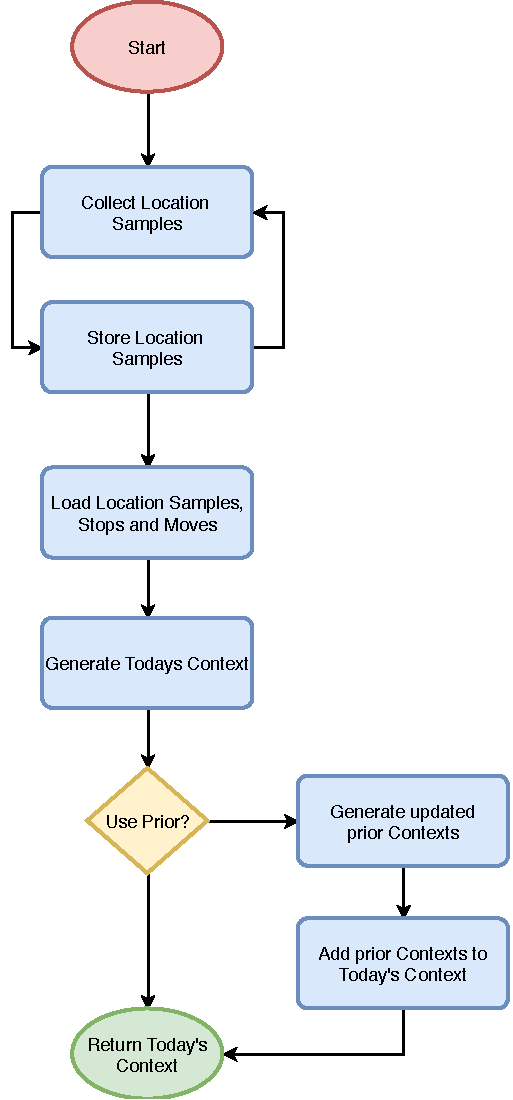
\includegraphics[width=0.5\textwidth]{images/diagrams/api-flowchart.pdf}
    \caption{The flowchart for computing mobility features using historical data}
    \label{fig:flowchart-features}
\end{figure}



\section{System Design}
The core idea of the \textit{Mobility Feature Package} is to provide a very simple programming interface such that computing features can be done with very few lines of code. This requires closing of the internal working of the package off, such that the programmer has very limited ways in which he/she can interface with it. The design of the package API went through two main iterations which consisted of many smaller iterations. Mainly, the difference between the final iteration and the earlier iterations is the amount of code required for managing historical data that the programmer has to write. Early iterations put the responsibility on the application programmer to manage historical data. After developing the field study app discussed in chapter \ref{chapter:06} it was decided to move most of this logic inside the package; it became glaringly apparent that the package was too cumbersome to use. The final iteration is the one discussed in this thesis including the choices and lessons learned on the way of designing and developing it. The flowchart in Figure \ref{fig:flowchart-features} displays the task which the software system must be able to carry out.

\begin{figure}
    \centering
    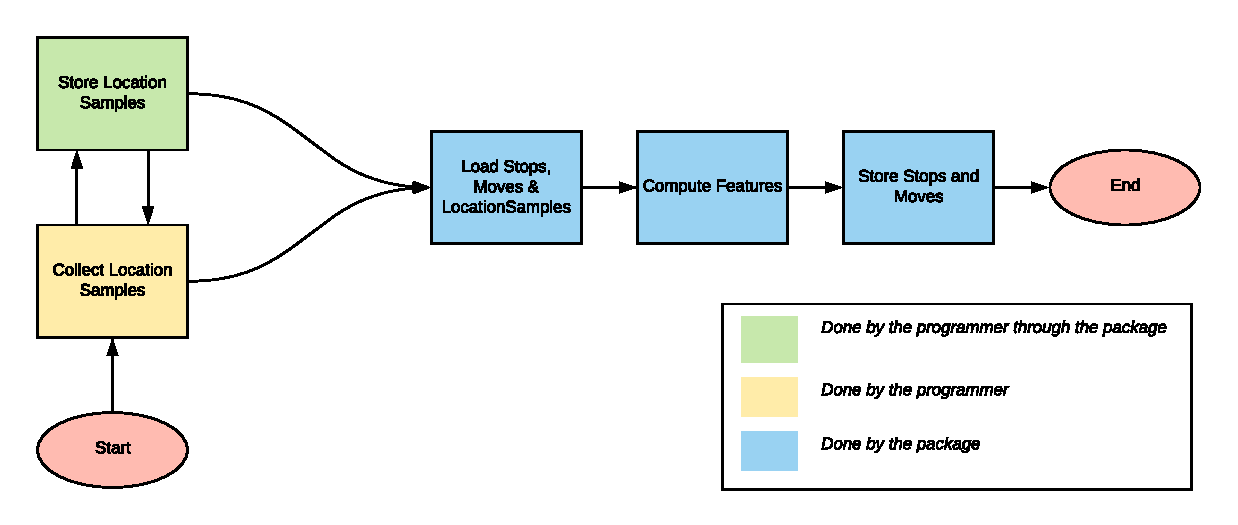
\includegraphics[width=0.5\textwidth]{images/diagrams/flowchart.pdf}
    \caption{Flowchart of the feature computatation process}
    \label{fig:my_label}
\end{figure}


\subsection{Component Overview}
Figure \ref{fig:component-diagram-internal} displays how the final iteration looks like as a software system: The main component is the \textit{Context Generator} component which is the interface that the programmer will use. This component exposes two interfaces to the programmer allowing the user to store their collected \textit{LocationSamples} as well as generate a \textit{Mobility Context} that contains the daily features. The two exposed interfaces are provided by the programmer through mobile application. The \textit{Context Generator} is also responsible for storing and loading data via the \textit{Mobility Serializer} component, here the \textit{Serializable} type refers to any data type that needs to be stored as historical data.

\begin{figure}[h]
\centering
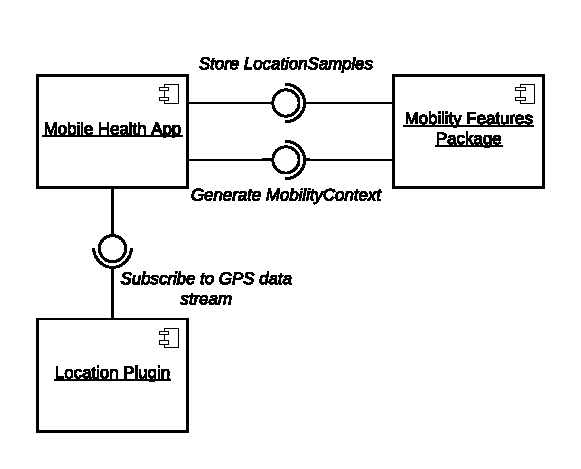
\includegraphics[width=0.5\textwidth]{images/diagrams/component-external.pdf}
\caption{Component diagram for the \textit{Mobility Feature Package} from an internal point of view}
\label{fig:component-diagram-internal}
\end{figure}

Figure \ref{fig:component-diagram-external} shows the external software system that includes the mobile application using the package. Another design choice is reflected in this figure which is the usage of an external location plugin which must be done by the programmer. This means task the programmer has to collect their own location data through their location plugin which will collect location \textit{Data Transfer Objects} (DTOs) \cite{fowler-PEEA} [p. 401]. These objects hold location data, i.e. latitude, longitude, and a timestamp and can be converted to \textit{LocationSamples} and saved through the \textit{Mobility Feature Package.}
Two reasons led to this decision, the first of which being that the Mobility Features Package becomes more loosely coupled and modular. The second reason relates to maintenance; if the package was to implement location data collection then it becomes harder to maintain since any change to the location plugin would imply changes to the Mobility Features Package as well. 

\begin{figure}[h]
\centering
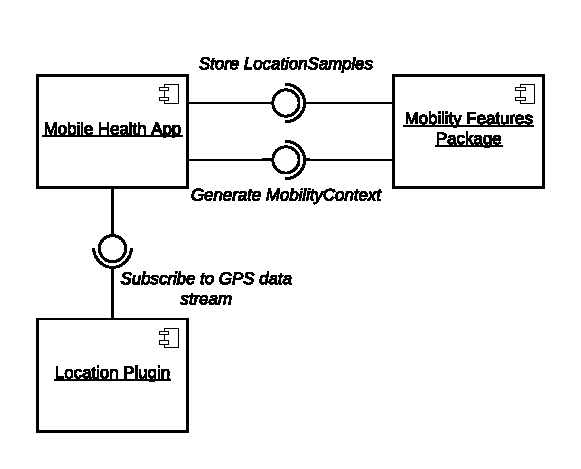
\includegraphics[width=0.5\textwidth]{images/diagrams/component-external.pdf}
\caption{Component diagram for the \textit{Mobility Feature Package} from an internal point of view}
\label{fig:component-diagram-external}
\end{figure}


\subsection{Sequence Overview}
To display the interactions between the components, sequence diagrams are used. Figure \ref{fig:sequence-diagram-external} shows the system from an external point of view, where the application subscribes to location updates via the location plugin, saves location data via the Mobility Features Package and generates a Mobility Context through it. 

\begin{figure}[h]
\centering
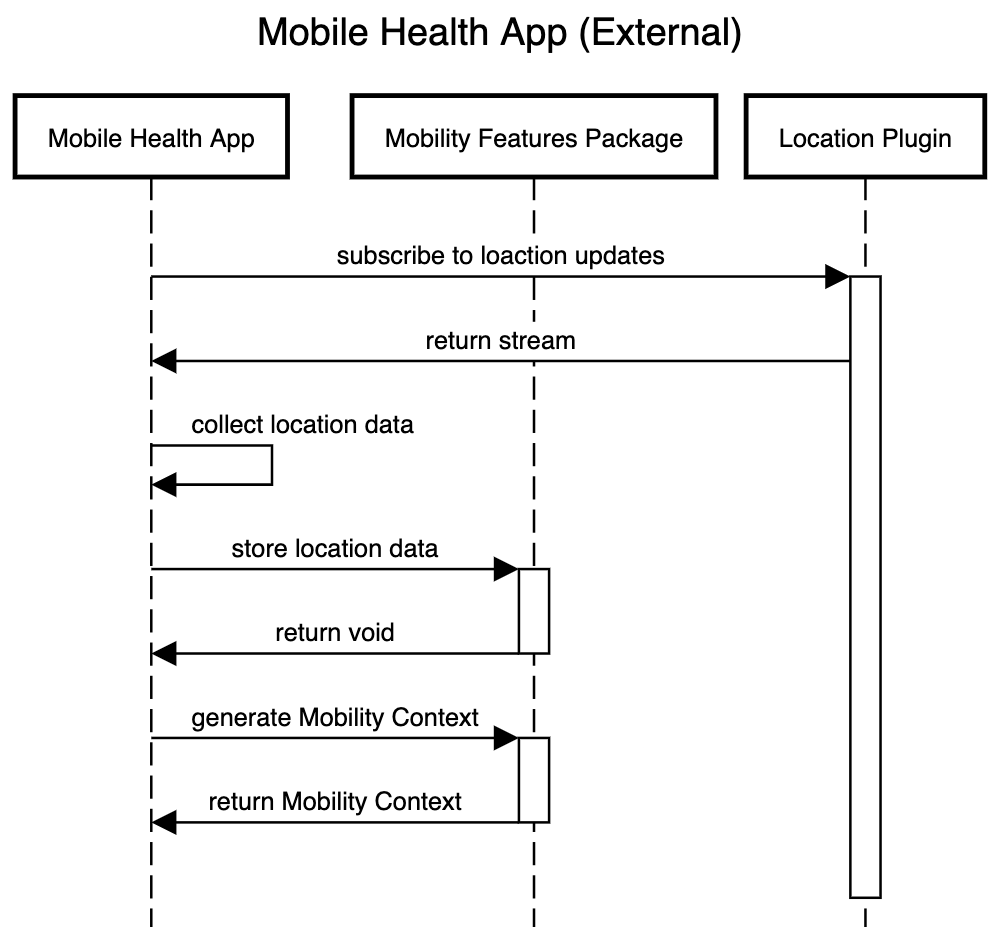
\includegraphics[width=0.7\textwidth]{images/diagrams/sequence-external.png}
\caption{Component diagram for the \textit{Mobility Feature Package} from an internal point of view}
\label{fig:sequence-diagram-internal}
\end{figure}

From an internal point of view, the \textit{Context Generator} component calls the \textit{Mobility Serializer} for storing and loading historical data, uses the loaded data to generate a \textit{Mobility Context} by calling the MobilityContext component.
\begin{figure}[h]
\centering
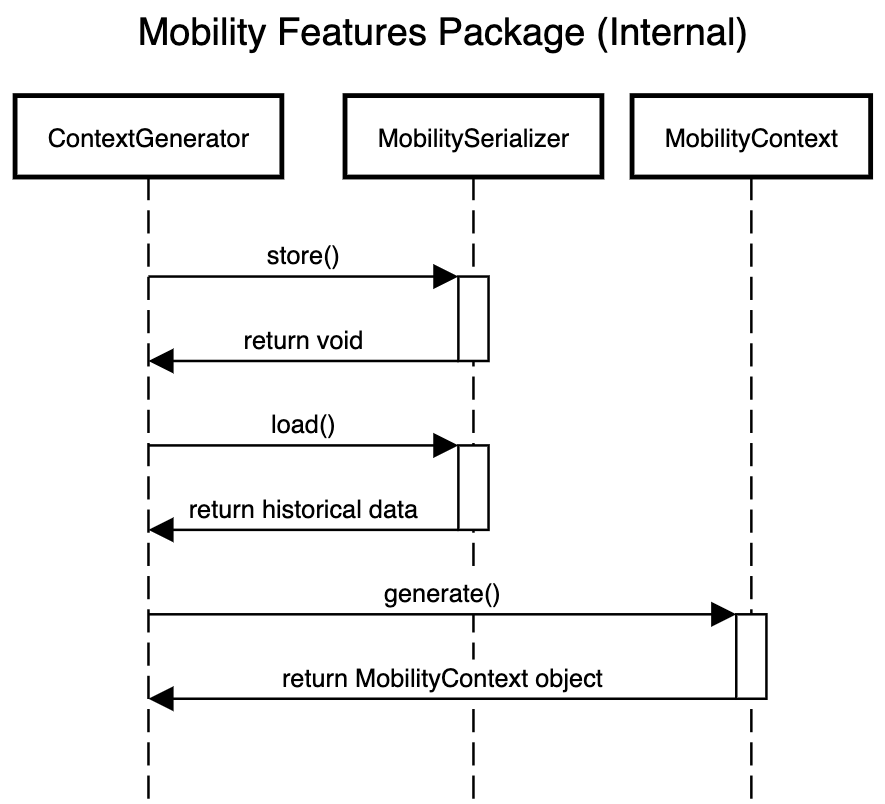
\includegraphics[width=0.7\textwidth]{images/diagrams/sequence-internal.png}
\caption{Sequence diagram for mobile health application using the Mobility Features Package, i.e. viewed externally from the package}
\label{fig:sequence-diagram-external}
\end{figure}
\section{Domain Model}
The domain model provides clarity and direction for a software system, even on a small scale such as in a library. In this section the design choices of the data model will be discussed.

\subsection{Data Model Overview}
In order to capture the data model in an object-oriented programming language, a UML diagram was maintained as the implementation went along in order to keep track of relationships between the classes. 
% As a general rule of thumb, all the fields were made public including those required by the constructors, and the methods of the classes were all \textit{getters}, i.e. \\

\subsubsection*{GeoPosition}
A \textit{GeoPosition} is defined by a geographical \textit{latitude} and \textit{longitude} and represents a 2D position on the Earth's surface.

\subsubsection*{Location Sample}
A \textit{Single Location Data Point} is a time-stamped \textit{Location}. By having a time-stamp, a collection of Location Samples may be ordered and grouped by the time of day. In essence, the class is a Data Transfer Object (DTO) \footnote{\url{https://martinfowler.com/eaaCatalog/dataTransferObject.html}} which is used to transfer GPS data from an arbitrary Location plugin to the \textit{Mobility Features Package}.

\subsubsection*{Hour Matrix}
An \textit{Hour Matrix} is a matrix with 24 rows and columns equal to the number of places of some period. The \textit{Hour Matrix} class is used to calculate the \textit{Routine Index} feature, as well as to identify the \textit{Home Cluster}, which is the place most visited during 00:00 and 06:00. An Hour Matrix is constructed from a list of \textit{Stops} which all have the same date.

\subsubsection*{Stop}
A \textit{Stop} is constructed from a centroid of a data point cluster (i.e. a Location) in addition to an arrival- and a departure timestamp, and a place ID indicating which place it belongs to.

\subsubsection*{Place}
A \textit{Place} is constructed from a place ID, as well as a collection of \textit{Stops} belonging to that \textit{Place}. 

\subsubsection*{Move}
A \textit{Move} is constructed from a pair of \textit{Stops} as well as the set of \textit{LocationSamples} which were sampled in between the two \textit{Stops} which is the path the user took between the two \textit{Stops}.

\subsubsection*{Mobility Context}
A \textit{Mobility Context} is a collection of features which are derived from a set of intermediate features, where the \textit{Stops} and \textit{Moves} are from a specific date. The \textit{Places} is derived from multiple dates for reasons which will be explained in the implementation details. In addition, a set of \textit{Mobility Contexts} from previous dates can be provided as an optional parameter. A Mobility Context contains the mobility features, although the \textit{Routine Index} is only available if an array of the set of \textit{Mobility Contexts} was provided as a parameter, which is due to the feature depending on the data from previous days in order to compare them.

\subsubsection*{GeoSpatial (Interface)}
This interface will impose a getter-method for the GeoPosition of the class which implements it. This allows the Haversine distance to be calculated between objects of different types.

\subsubsection*{Serializable (Interface)}
This interface will impose a serialization and de-serialization method for converting between a language object and a JSON object. The interface will allow the MobilitySerializer component as previosly discussed to more easily implement serialization in a generic manner which is disucssed in Chapter \ref{chapter:05}.

\subsection{UML Diagram and Discussion}

\begin{figure}[h]
    \centering
    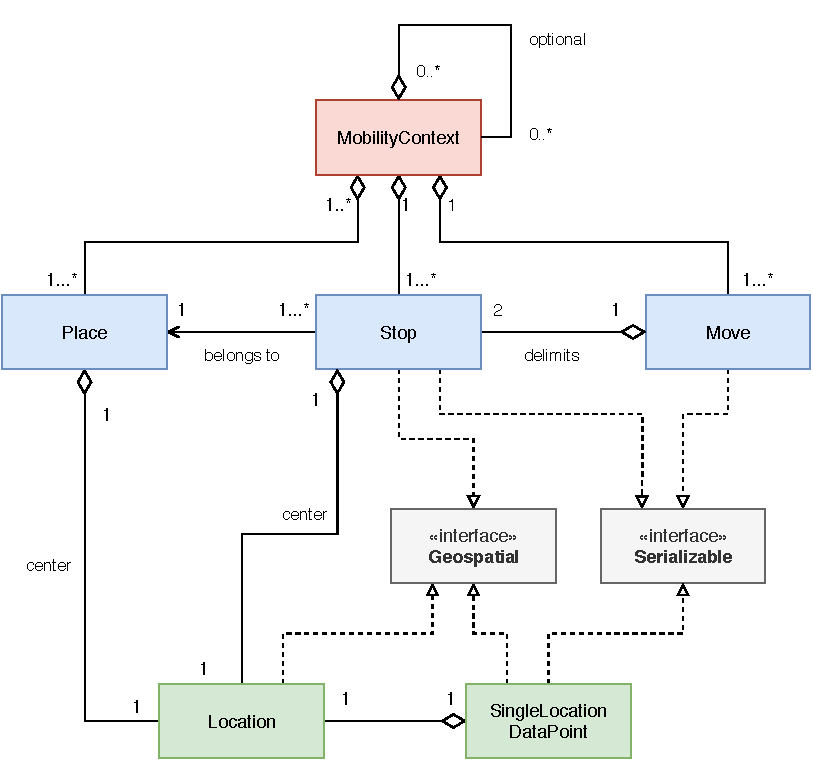
\includegraphics[width=0.7\textwidth]{images/diagrams/uml.pdf}
    \caption{UML diagram for the classes used in the \textit{Mobility Features Package}}
    \label{fig:my_label}
\end{figure}

The data model could be modified such that a Place contained a list of \textit{Stops} made at that place, rather than using both \textit{Places} and \textit{Stops} for instantiation of \textit{Mobility Context}. This would mean grouping the \textit{Stops} by Place rather than date, and would require filtering to take place every time a \textit{Mobility Context} object is created, to remove all Stops, not on that specific date. In a real-world scenario the application developer will likely have the Location Samples for the current day available, and from those the \textit{Stops} today can be generated which means no filtering is required. Grouping \textit{Stops} into places would however lead to a nicer data model, but a design choice was made in favor of less computation. 




